\documentclass[conference]{IEEEtran}

%%%% Bibtex then pdfLatex

\usepackage{cite}
\usepackage{graphicx}
\usepackage{hyperref}
\usepackage{listings}
\usepackage{times}
\usepackage{xspace}
\usepackage{booktabs}
\usepackage{subfigure}
\usepackage{fancybox}
\usepackage{color}
\usepackage{multirow}
\usepackage{array}
\usepackage{subfigure}
\usepackage{balance}
\usepackage{tabularx}
\newcommand{\todo}[1]{\colorbox{yellow}{\textbf{[#1]}}}
\newcommand{\emad}[1]{\textcolor{red}{{\it [Emad says: #1]}}}
\newcommand{\dan}[1]{\textcolor{blue}{{\it [Dan says: #1]}}}


\hyphenation{op-tical net-works semi-conduc-tor}


\begin{document}
%
% paper title
% can use linebreaks \\ within to get better formatting as desired
\title{CCCD: Concolic Code Clone Detection}


% author names and affiliations
% use a multiple column layout for up to three different
% affiliations
\author{\IEEEauthorblockN{Daniel E. Krutz and Emad Shihab}
Rochester Institute of Technology\\
\{dxkvse,emad.shihab\}@rit.edu

}


\maketitle


\begin{abstract}
%\boldmath
Code clones are multiple code fragments that produce similar results when provided the same input. Prior work has shown that clones can be harmful since they elevate maintenance costs, increase the number of bugs caused by inconsistent changes to cloned code and may decrease programmer comprehensibility due to the increased size of the code base.  

To assist in the detection of code clones, a number of tools have been proposed. Some of which include CCFinder, MeCC, CloneDR and Clonetracker. The majority of these tools depend on the syntactic similarities of code clones. However, a large number of code clones (e.g., Type-3 and Type-4 clones) contain a significant amount of syntactic differences. In this work we propose a new tool called Concolic Code Clone Detection (CCCD), which uses \emph{concolic analysis} to detect code clones. The advantage of this approach is that it discovers clones based on the functional not syntactic nature of the software. This means that numerous semantic issues which have plagued previous clone detection techniques do not have any adverse affects on CCCD. Based on our preliminary findings, CCCD has been highly effective in detecting clones of all types.
\end{abstract}


\IEEEpeerreviewmaketitle



\section{Introduction}

%Code clones exist
Code clones occur in software for a variety of reasons. Developers may knowingly duplicate functionality across the software system. This may be due to an unwillingness to refactor and retest the modified portion of the application, or simply due to laziness on the part of the developer. Clones continue to be extremely widespread in software development. It is estimated that clones comprise between 5-23\% of all source code \cite{Baxter:1998:CDU:850947.853341} \cite{Schulze:2010:CCF:1942788.1868310}.


% They make code hard to maintain, so tools are needed.
A significant amount of previous work states that code clones are undesirable \cite{Mondal:2012:ESC:2387358.2387360} \cite{Duala-Ekoko:2010:CRD:1767751.1767754}. One of the most prominent reasons against code clones is that they substantially raise the maintenance costs associated with an application~\cite{Juergens:2009:CCM:1555001.1555062}. Reducing maintenance costs is a very serious matter since the maintenance phase of a project has been found to comprise between 40-80\% of the cost of a software project \cite{Shukla:2008:ESM:1342211.1342232} \cite{Ducasse:1999:LIA:519621.853389} \cite{SMR:SMR225} \cite{Ueda:2002:GMS:823457.824039}. Finally, unintentionally making inconsistent bug fixes to cloned code across a software system is also likely to lead to further system faults \cite{Deissenboeck_2010}. 


Clone detection tools have been proposed to assist practitioners in detecting code clones so they may be easily detected. Such code clone tools have helped in discovering clone-related bugs and even security vulnerabilities in software systems~\cite{Dang:2012:XTC:2420950.2421004}.

There are four types of code clones which are generally recognized by the research community. Type-1 clones are the simplest and represent identical code except for variations in whitespace, comments and layout. Type-2 clones are syntactically similar except for variations in identifiers and types. Type-3 clones are two segments which differ due to altered or removed statements. Type-4 clones are the most difficult to detect and represent two code segments which considerably differ syntactically, but produce identical results when executed \cite{Gold:2010:ICC:1808901.1808916}. 


There are numerous tools which discover clones in a variety of ways. While many are able to discover the simpler type-1 and type-2 clones, fewer have the ability to find type-3 and type-4 clones. Type-4 clones are typically the most difficult clones to detect and may be more problematic than type-1, type-2 and type-3 clones  \cite{Roy07asurvey}. To the best of our knowledge, only two known techniques are able to discover the most complicated types of clones, type-4 \cite{Roy:2009:CEC:1530898.1531101, Kraw2012}. 

In this paper, we propose Concolic Code Clone Detection (CCCD), a tool for finding code clones which uses \emph{concolic analysis} as a driving force for discovering clones. Concolic analysis combines concrete and symbolic values in order to traverse all possible paths (up to a given length) of an application. Concolic analysis has been traditionally used in software testing to find faults in an application \cite{Kim:2012:IAC:2337223.2337373}. Concolic analysis forms the basis for a powerful clone detection tool because it only considers the functionality of the source code and not its syntactic properties. This means that things such as comments and naming conventions which have been problematic for existing clone detection techniques will not affect concolic analysis and its discovery of clones. This tool is innovative for several reasons. First, only two other works claim the ability to discover type-4 clones, with each having some drawbacks.   Additionally, it represents the only known proposed technique for discovering clones which is based upon concolic analysis.

While CCCD is not perfect, its ability to reliably discover type-4 clones is profound. Using clone benchmarks defined by prior research, CCCD was able to detect the majority of code clones (of all types) in both a single file as well as clones which were injected into several open source software applications.


% The remained of the paper is organized as follow..
The rest of the paper is organized as follows. Section~\ref{sec: CCCD_tool} provides an overview of the proposed CCCD tool. Section~\ref{sec: implementationandeval} discusses the primary components of CCCD and how it was validated. Section~\ref{sec: relatedwork} briefly describes existing clone detection tools and some of the current uses of concolic analysis. Section~\ref{sec: conclusion} summarizes the findings and conveys future work to be done on CCCD, including some future applications of this tool.

\section{The CCCD Tool}
\label{sec: CCCD_tool}
CCCD follows a traditional pipe-and-filter architecture. Figure~\ref{fig:cccdstructure} shows the basic components of the CCCD tool. CCCD is comprised of two primary phases. First a Unix bash script generates the necessary information for analysis. The concolic output is generated using an open source tool known as CREST \cite{Burnim:2008:HSD:1642931.1642995}. The process of identifying code clone candidates is done using a comparison component written in Java and is invoked automatically from the Unix bash script. Even though specific tools are described in the implementation of CCCD, these components are all easily interchangeable and newer or more robust technologies may be added to the tool as needed. The final report contains a listing of all code clone candidates as identified by CCCD.

\begin{figure}[thb!]
\centering
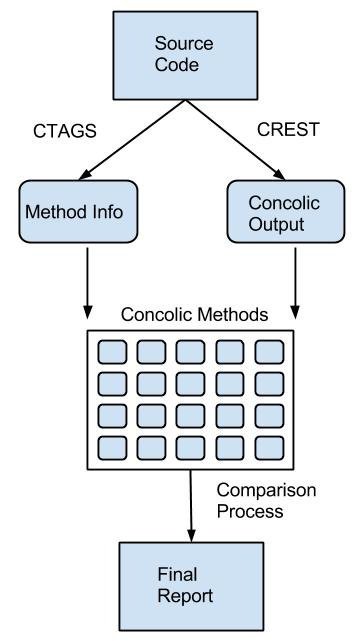
\includegraphics[width=33mm,height=60mm]{images/CCCDStructure_2.jpg}
\caption{Overview of the CCCD Tool}
\label{fig:cccdstructure}
\end{figure}



\subsection*{Data Generation}
The initial step of CCCD is to generate the required information for analysis. An open source tool known as CREST was selected for generating the necessary concolic output. This tool was chosen because it is highly configurable, open source and robust. The bash component of CCCD first loops through the source code of the target application. CREST is executed against all source code files with a .c extension. The generated concolic output is stored in external text files for further analysis. 

A goal of this clone detection tool is to discover code clone candidates at the method level. The next step is to separate the generated concolic output for each targeted class and create a separate file containing the concolic output of each method. In order to note the methods in the source code for each class, an application known as CTAGS \footnote{http://ctags.sourceforge.net} is used. This tool is able to quickly and efficiently note the methods in the source code for the target application. This method information is stored in an external file and is used to break the concolic output for each class into individual files for all methods inside of the class. 


\subsection*{Comparison Process}

Once all of the necessary data has been created (i.e., the conconlic analysis is run on the code), the comparison portion of the tool is then invoked to process this information and ultimately identify any code clone candidates. Using the generated information from CTAGS, the concolic output for each class is broken up for each method and is stored in a newly created file. Each method in the entire application will have an external file created for it.

After all of the concolic method files have been created, the comparison process begins. The goal is to record similar concolic output for any of the methods. This is accomplished by comparing each concolic output method file against others in a round robin fashion. In order to measure the similarity between two files, the Levenshtein distance measurement is used. The Levenshtein distance is defined as the minimal number of characters that would need to be replaced in order to convert one string to another \cite{Bard:2007:STO:1274531.1274545}. While there are other string similarity techniques which may be viable options, the Levenshtein distance metric was found to be well suited for this clone detection task. In order to help normalize the similarity results based on length, the final Levenshtein score (ALV) is computed by dividing the Levenshtein distance between two files (LD) by the longest string length of the two strings being compared (LSL) and then multiplying by 100.  The ALV formula is shown below in Equation~\ref{eq:avglevenformula}.
%with the key represented in Table ~\ref{table:avgLevenshteinFormulaKey}.


\begin{equation} \label{eq:avglevenformula} 
ALV = (LD/LSL) \times 100     
\end{equation}




%\begin{table}[thb!]
%\begin{center}
%    \begin{tabular}{ l | l}
%    \toprule
% 	ALV & Calculated Average Levenshtein Value \\ \hline
%	LD & Levenshtein distance between two strings \\ \hline
%	LSL & Longest String Length between to analyzed strings \\
%	\bottomrule
%	
%    \end{tabular}
%\end{center}
%
%\caption{Avg. Levenshtein Formula Key}
%\label{table:avgLevenshteinFormulaKey}
%\end{table}



The results of each comparison are stored in a final report .csv file. In order to make the generated information more manageable for the user, only comparisons with a Levenshtein score of 35 or less are added to the report. This is because our preliminary empirical analysis showed that comparisons with a distance of 35 or less yielded higher quality code clone candidates. More analysis is needed to determine the impact of the  Levenshtein score on the performance of the CCCD tool. A brief representation of the output is shown in the Appendix (Table~\ref{table:exampleresults}).


The tool and complete results may be found by visiting the main project website at \url{http://www.se.rit.edu/\~dkrutz/CCCD/}.

\section{Implementation and Evaluation}
\label{sec: implementationandeval}


In order to evaluate CCCD, we first compare its performance on the code clone benchmarks provided by Krawitz\cite{Kraw2012} and Roy\cite{Roy:2009:CEC:1530898.1531101}. In their work, each of Krawitz and Roy defined benchmarks containing clones of all four types and laid out several explicit examples of each type. The initial step was to ensure that CCCD would be able to detect all of these predefined clones individually. A simple C application was created which contained the sixteen clones as defined by Roy and four as defined by Krawitz. 

Several methods were inserted into this class which were not clones of any other methods in the class. The purpose of this was to help ensure that CCCD did not incorrectly identify methods to be clones which were not. This class was then analyzed by CCCD. Out of 465 comparisons, 296  were manually determined not to be comparisons between two methods which represented clones while 165 comparisons were manually determined to represent code clones. CCCD was then ran against the target source code. Comparisons with a Levenshtein similarity score of under 35 were deemed to be code clone candidates. These values were selected after several previous test runs with this source code, along with the source code from other applications.

CCCD was able to determine whether or not two methods were clones with an accuracy of 93\%. An additional, 17 comparisons were  recommended for further manual analysis (i.e., had a Levenshtein score close to 35). Another 14 comparisons should have been identified as clones, but were not. This is not considered to be overly concerning for CCCD. All of these non-identified clones were type-4 clones from the work by Krawitz. This was likely a problem that CCCD had with the specific type of clone method as laid out by Krawitz. Additionally, CCCD was able to identify the remaining type-4 clones as presented in the work by Roy. There were no false positives, meaning that all clone candidates identified by CCCD were manually verified to be actual clones. 

Another interesting finding is the wide gap between methods which were clones and methods that were not clones. Methods which were manually identified as clones had an average Levenshtein similarity score of  12.7 while non-clones had a much higher average score of 58.4. A listing of the results is shown in Table ~\ref{table:completeKrawresults}. A more thorough list of the results may be found on the project website. 


%%% Numbers do not exactly match up because...
%%% - Clean up the results and put them on the website



\begin{table}[thb!]
\begin{center}
    \begin{tabular}{ l | l }
    \toprule
 	Total Comparisions & 465 \\ \hline
	Not clones & 296 (65\%) \\ \hline
	Clones & 165  (35\%)  \\ \hline
	Correctly Identified & 434 (93\%) \\ \hline
	Not Identified & 14  (3\%) \\ \hline
	Recommended & 17  (3.5\%) \\ \hline
	False Positive & 0  (0\%) \\ \hline
	Avg. Leven Clones & 12.7 \\ \hline
	Avg. Leven Non-Clones & 58.4 \\ \bottomrule

    \end{tabular}
    \caption{Clone Detection Results}
    \vspace{-0.2in}
\end{center}


\label{table:completeKrawresults}
\end{table}



The next phase was to ensure that these clones could be discovered in existing systems. Several open source applications were selected for this analysis. These included FileZilla \footnote{https://filezilla-project.org}, VLC \footnote{http://www.videolan.org} and MySQL \footnote{http://www.mysql.com}. Each of the predefined clones taken from the works of Roy and Krawitz were randomly inserted into the source code of these applications with their locations being noted. A complete listing of the results is shown in Table~\ref{table:injectedclones}.


\begin{table}[thb!]

\begin{center}
    \begin{tabular}{ l | l | l | l | l | l }
    \toprule
    Application & Type-1 & Type-2 & Type-3 & Type-4 & Total \\ \hline
    VLC  & 5/5  &6/6   & 7/7  & 6/8  & 24/26 (92\%)\\ \hline
MySQL & 5/5  &6/6   & 7/7  & 6/8  & 24/26 (92\%)\\ \hline
FileZilla & 5/5  &6/6   & 7/7  & 6/8  & 24/26 (92\%)\\ \bottomrule

    \end{tabular}
\end{center}
\caption{Results of the Injected Clones by CCCD}
\label{table:injectedclones}
\vspace{-0.3in}
\end{table}




CCCD was able to discover these clones with similar results as in the previously described control class. This analysis shows that concolic analysis used in CCCD is the same for each method, regardless of where it resides and its surrounding methods. The comparison process will therefore return similar results for these methods, regardless of what application they reside in. 



\section{Related Work}
\label{sec: relatedwork}

There are numerous clone detection tools which utilize a variety of methods for discovering clones. Some of which include text, lexical, semantic, symbolic and behavioral based approaches \cite{Roy:2009:CEC:1530898.1531101}. Only two known works claim the ability to reliably detect type-4 clones. MeCC discovers clones based on the ability to compare a program's abstract memory states. While this work was successful in finding type-4 clones, this tool suffers from several drawbacks including the ability to only analyze pre-processed C programs and an excessive clone detection time which is likely caused by the exploration of an unreasonably large number of possible program paths \cite{Kim:2011:MMC:1985793.1985835}.  Krawitz \cite{Kraw2012} proposed a clone discovery technique based on functional analysis. This process was shown to detect clones of all types, but was never implemented into a reasonably functional tool. Additionally, this technique requires a substantial amount of random data which may be a difficult and time consuming process to produce.


\section{Conclusion and Future Work}
\label{sec: conclusion}

CCCD has been shown to be a new, robust and effective technique for clone discovery. Preliminary work has demonstrated its effectiveness in discovering clones of all four types. This includes type-4 clones, which only two other techniques purport the ability to locate.

While a tool that employs concolic analysis as its driving force and is able to discover type-4 code clones is profound, there are significant opportunities for future work. CCCD will first be compared against existing leading clone detection techniques. Likely candidates include MeCC, CCFinder \cite{Kamiya:2002:CMT:636188.636191} and Deckard \cite{Jiang:2007:DSA:1248820.1248843}. CCCD is likely able to find more type-4 clones than Deckard and CCFinder since previous research has noted these tools to struggle at finding the more complicated types of clones. Some of the reasons for the struggles include the inability to overcome semantic differences in the source code or problems with normalization \cite{Roy07asurvey}.

Currently, CCCD only analyzes files with a .c extension. Source code located in other files, including .h, were not examined. In the future, CCCD will be expanded to explore these file types in order to discover clones in a wider spectrum of file types. Furthermore, future work will be done to analyze much larger data sets using CCCD and compare this new and innovative technique against leading existing clone detection tools. CCCD will also be applied in answering questions of how clones affect the software development and maintenance process. 




%%% Other Future work
% - Proper depth search
% -  Speed things up.




%\bibliographystyle{ieeetr}
%\bibliography{IEEEabrv,paper,refs}

\vspace{-0.2in}
\bibliographystyle{plain}
\bibliography{refs}



\appendix
\label{sec: appendix}

CCCD is an open source tool and may be downloaded in a Fedora 14 Virtual Machine at \url{http://www.se.rit.edu/~dkrutz/CCCD/}. The complete source code for the tool may be found in a public SVN repository at \url{http://code.google.com/p/dk-crest-java/}. The following section describes the steps required to run CCCD.\\


\section{Installation}
{\bf A. Installation} % Fix this formatting%

The simplest way to attain CCCD is to download the Fedora 14 VM which CCCD is already configured and installed on. If the user wants to install CCCD in their own environment, they should download and install the following into their Linux environment:

\begin{enumerate}
 \item CREST
  \item CTAGS
 \item Java 1.6
  \item CCCD
\end{enumerate}

Users taking this approach should refer to the component's respective website for installation assistance. Other packages required by these components may also need to be installed depending on the specific environment chosen by the user. CIL is a required component of CREST and will need to be slightly modified. In the cil/src directory, the file cil.ml will need to replaced by a modified version for CCCD. This modified version of the file, along with instructions, may be found in the public SVN under bashScripts/customfiles. CCCD may be installed by merely retrieving its latest build from its public SVN repository and placing the attained file structure under the user's HOME directory.

While CCCD will run in a variety of Unix and Unix-like environments, it has only been tested in Fedora 14 running Java 1.6. The primary environmental limiting factor for CCCD is the environments that CREST and CTAGS are able to properly run in. \\


\section{Data Population}
{\bf B. Data Population} % Fix this  formatting%

CCCD is able to process C based source code in its search for clones. No pre-processing is required. To begin the clone detection process, the user should place the raw source code in the sourceFiles/input/\{appname\} directory. Examples of this are represented in Figure ~\ref{fig:initialimportfolder} and Figure ~\ref{fig:initialimportfolder_terminal} assuming that "kraw" was the source file to be analyzed.



\begin{figure}[t!]
\centering
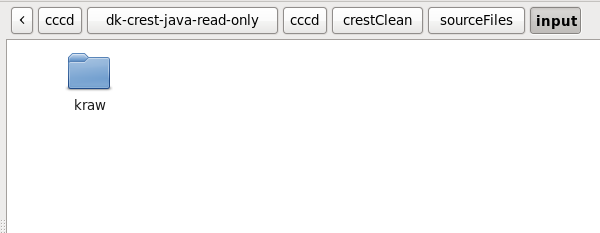
\includegraphics[width=85mm,height=40mm]{images/initialinputfolder.png}
\caption{Inital Input Folder Example \#1}
\label{fig:initialimportfolder}
\end{figure}


\begin{figure}[t!]
\centering
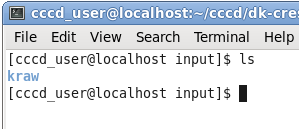
\includegraphics[width=50mm,height=20mm]{images/input_terminal.png}
\caption{Inital Input Folder Example \#2}
\label{fig:initialimportfolder_terminal}
\end{figure}


Since the CREST component of CCCD will attempt to analyze each C file individually, all necessary header files which are not located in the same directory as the file being analyzed need to be included as environmental variables. This may be 
done by using the "export C\_INCLUDE\_PATH" command in Unix. More information on this command may be found at:
\url{http://www.network-theory.co.uk/docs/gccintro/gccintro_23.html}. Another example of this command is shown in Figure ~\ref{fig:exportcommand} \\



\begin{figure}[t!]
\centering
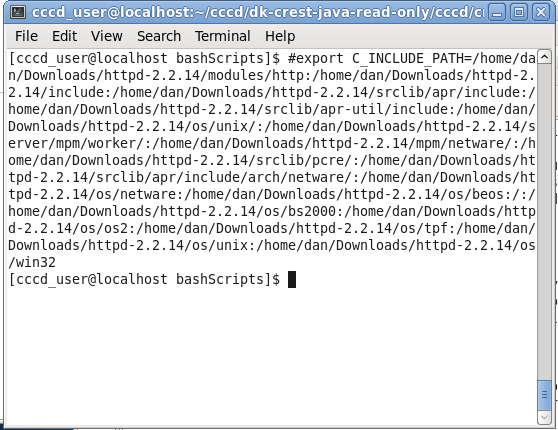
\includegraphics[width=90mm,height=65mm]{images/exportcommand.png}
\caption{Export\_C Command}
\label{fig:exportcommand}
\end{figure}



\section{Running CCCD}
{\bf C. Running CCCD} % Fix this  formatting%


Once the application to be examined has been copied to the appropriate input directory, CCCD may be executed. This is done by executing the following command from the bashScripts directory:
\begin{lstlisting}
bashScripts$ ./cccd \{appname\}
\end{lstlisting}

An example of this command may be viewed in Figure~\ref{fig:executecommand} 



\begin{figure}[t!]
\centering
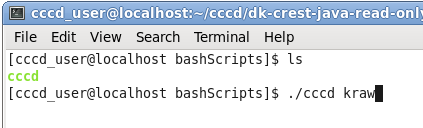
\includegraphics[width=50mm,height=22mm]{images/beforeexecution_terminal.png}
\caption{CCCD Execute Command}
\label{fig:executecommand}
\end{figure}


The appname parameter should exactly match the name of the folder which the source code was placed into in the sourceFiles/input directory. Once this command is invoked, the application will begin. Screen output will include information regarding file directories being generated, CREST and CTAGs information being created, the method comparisons and ultimately with the location of the final report. Depending on the size of the source code being analyzed, this entire process may take a few seconds to a few hours. An example of CCCD during execution may be viewed in Figure ~\ref{fig:cccdrunning} \\


\begin{figure}[t!]
\centering
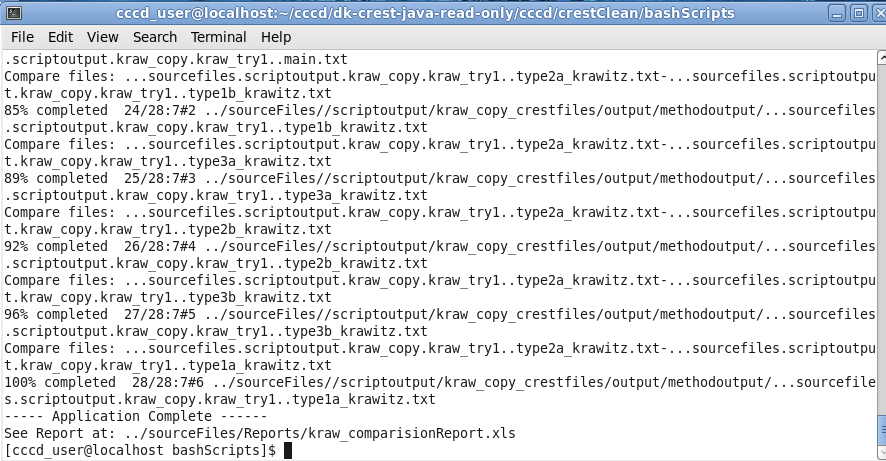
\includegraphics[width=90mm,height=65mm]{images/finaloutput.png}
\caption{CCCD Execution Window}
\label{fig:cccdrunning}
\end{figure}

\section{Viewing Reports}
{\bf D. Viewing Reports} % Fix this  formatting%


The final report in .csv format may be viewed at sourceFiles/Reports/appname.csv . The report contains all method comparisons which were conducted using the computed Levenshtein average. Comparisons over this average are not shown in order to significantly reduce the amount of information displayed to the user and are comparisons which are highly unlikely to be code clones. The report is shown in the following format:



\begin{table}[t!]
\begin{center}
  %%%%  \begin{tabular}{| p{3cm} | l |}
  \begin{tabular}{| l | l |}
    \hline
    Files & Leven Avg. Distance \\ \hline

	kraw/type1a\_krawitz()-kraw/type1b\_krawitz()& 0 \\ \hline
	kraw/type2a\_krawitz()-kraw/type1a\_krawitz()& 11 \\ \hline
	kraw/type2a\_krawitz()-kraw/type1b\_krawitz()& 11 \\ \hline
	kraw/type2b\_krawitz()-kraw/type1a\_krawitz()& 1 \\ \hline
	kraw/type2b\_krawitz()-kraw/type1b\_krawitz()& 1 \\ \hline


    \end{tabular}
\end{center}

\caption{Example Results Set}
\label{table:exampleresults}
\end{table}

Table ~\ref{table:exampleresults} represents the final result set created by CCCD. The first column displays the two methods which are compared with each other. The final column displays the calculated average Levenshtein distance. 




% that's all folks
\end{document}





%%% Emad
% - Fix broken references (If they exist)
% - Fix format of appendix.
% - Fix any other formatting issues.
% - Proofread all substantially.


%%%%% Todo:
% - Fix appendix line breaks
% - Mention why counts are off
% - Ensure that the website is squared away
